% \documentclass[12pt]{article}
\documentclass[12pt]{scrartcl}
\title{EM-Pertemuan 7}
\nonstopmode
%\usepackage[utf-8]{inputenc}
\usepackage{graphicx} % Required for including pictures \usepackage[figurename=Figure]{caption} \usepackage{float}    % For tables and other floats
\usepackage{verbatim} % For comments and other
\usepackage{amsmath}  % For math
\usepackage{amssymb}  % For more math
% \usepackage{amsfonts} % For more math fonts
\usepackage{fullpage} % Set margins and place page numbers at bottom center
\usepackage{paralist} % paragraph spacing
\usepackage{listings} % For source code
\usepackage{subfig}   % For subfigures
%\usepackage{physics}  % for simplified dv, and 
\usepackage{enumitem} % useful for itemization
\usepackage{siunitx}  % standardization of si units
\usepackage{esint}
\usepackage{tikz,bm} % Useful for drawing plots
%\usepackage{tikz-3dplot}
\usepackage{cancel}
% \usepackage[a4paper, margin=1cm ]{geometry}
%%% Colours used in field vectors and propagation direction
\definecolor{mycolor}{rgb}{1,0.2,0.3}
\definecolor{brightgreen}{rgb}{0.4, 1.0, 0.0}
\definecolor{britishracinggreen}{rgb}{0.0, 0.26, 0.15}
\definecolor{cadmiumgreen}{rgb}{0.0, 0.42, 0.24}
\definecolor{ceruleanblue}{rgb}{0.16, 0.32, 0.75}
\definecolor{darkelectricblue}{rgb}{0.33, 0.41, 0.47}
\definecolor{darkpowderblue}{rgb}{0.0, 0.2, 0.6}
\definecolor{darktangerine}{rgb}{1.0, 0.66, 0.07}
\definecolor{emerald}{rgb}{0.31, 0.78, 0.47}
\definecolor{white}{rgb}{255, 255, 255}
\definecolor{palatinatepurple}{rgb}{0.41, 0.16, 0.38}
\definecolor{pastelviolet}{rgb}{0.8, 0.6, 0.79}


% special config
\usepackage{cleveref}
\usepackage[most]{tcolorbox}
\tcbset{
    boxrule=0pt,
    before=\noindent,
    sharp corners,
    enhanced jigsaw,
    % drop fuzzy shadow,
    breakable
}
% some auto vector etc.
\renewcommand{\epsilon}{\varepsilon}
\newcommand{\vnabla}{\vec{\nabla}}
\newcommand{\vE}{\vec{E}}
\newcommand{\vH}{\vec{H}}
\newcommand{\vB}{\vec{B}}
\newcommand{\vD}{\vec{D}}
\newcommand{\vJ}{\vec{J}}
\newcommand{\vr}{\vec{r}}
\newcommand{\vk}{\vec{k}}
\newcommand{\Curl}{\vec{\nabla}\times}
\newcommand{\Div}{\vec{\nabla}\cdot}

\newtcolorbox{answer}{
    beforeafter skip balanced=5pt,
    colback={white!97!ceruleanblue},
    borderline west={0.5pt}{0pt}{black!90!white},
}

% for arrow to the equation
\usepackage{calc}
\usepackage{tikz}
\usetikzlibrary{tikzmark,calc,,arrows,shapes, positioning,decorations.pathreplacing}
\tikzset{every picture/.style={remember picture}}
\usepackage{accents}
\newcommand\myubar[1]{%
\underaccent{\bar}{#1}}

% for EM wave img tikz
\usepackage{xcolor}
% \usepackage{physics}
\colorlet{myblue}{black!40!blue}
\colorlet{myred}{black!40!red}
\colorlet{vcol}{black}
\colorlet{Ecol}{black!90!black}
\colorlet{EVcol}{white!10!black}
\colorlet{Bcol}{black!70}

% for facny numbering without fancyhdr for CHAD
\usepackage[lastpage,user]{zref}
\renewcommand\pagemark{\usekomafont{pagenumber}\textbf{\thepage}\ of 9}

\begin{document}
\renewcommand{\figurename}{Figure}
\begin{center}
    \hrule
    \vspace{.4cm}
    \textbf{\large Elektromagnetika --- PR V}
\end{center}
\textbf{Nama}\hspace{1mm}: Firman Qashdus Sabil \hspace\fill \textbf{Offering:}\ AC\\
 \textbf{NIM}\hspace{3.3mm}: 210321606892 \hspace{\fill} \\%\textbf{Assignment:} Number 3 \\
\hrule

\begin{enumerate}[leftmargin=*]

    \item Menurunkan persamaan gelombang EM dengan kehadiran sumber, untuk medan $\vec{E}$.
    \begin{answer}
        Dari persamaan maxwell ke-3
\begin{equation*}
    \vnabla \times \vE = -\frac{\partial \vB}{\partial t}
\end{equation*}
Curl-kan kedua sis persamaan maxwell diatas,
\begin{align*}
    \vnabla \times \vnabla \times \vE &= \vnabla \times \left(-\frac{\partial \vB}{\partial t}\right)\\
    \vnabla \times \vnabla \times \vE &=  -\frac{\partial}{\partial t}\left(\vnabla \times \vB \right) 
\end{align*}
Dengan identitas vektor, bahwa $\vnabla \times \vnabla \times \vec{A}=\vnabla(\vnabla\cdot\vec{A})-\nabla^2 \vec{A}$ dan karena $\vB = \mu_0 \vH$ maka
\begin{align*}
    \vnabla(\vnabla\cdot\vec{E})-\nabla^2\vE=-\mu_0 \frac{\partial }{\partial t}\left(\vnabla \times \vH\right) 
\end{align*}
karena $\vnabla \times \vH = \frac{\partial \vD}{\partial t} + \vJ$ dengan $\vD = \epsilon_0 \vE$, maka
\begin{align*}
    \vnabla(\vnabla\cdot\vec{E})-\nabla^2\vE&=-\mu_0 \frac{\partial }{\partial t}\left(\vnabla \times \vH\right)\\
    &=-\mu_0 \frac{\partial }{\partial t}\left(\frac{\partial \vD}{\partial t}+\vJ\right) \\
    &=-\mu_0 \frac{\partial }{\partial t}\left(\epsilon_0\frac{\partial \vE}{\partial t}+\vJ\right) \\
    \vnabla(\vnabla\cdot\underbrace{\vec{E}}_{\dfrac{\vD}{\epsilon_0}})-\nabla^2\vE&=-\mu_0\epsilon \frac{\partial^2 }{\partial t^2}\vE-\mu_0\frac{\partial }{\partial t}\vJ
\end{align*}
Dalam kasus ini $\vnabla \cdot \vD = \rho; \text{dimana } \rho \neq 0$, sehingga
\begin{align*}
    \vnabla(\vnabla\cdot\frac{1}{\epsilon_0}\vD)-\nabla^2\vE&=-\mu_0\epsilon \frac{\partial^2 }{\partial t^2}\vE-\mu_0\frac{\partial }{\partial t}\vJ\\
    \frac{1}{\epsilon_0}\vnabla(\underbrace{\vnabla\cdot\vD}_{\rho})-\nabla^2\vE&=-\mu_0\epsilon \frac{\partial^2 }{\partial t^2}\vE-\mu_0\frac{\partial }{\partial t}\vJ\\
\end{align*}
karena $c=\dfrac{1}{\sqrt{\mu_0\epsilon_0}}$, maka
\begin{align*}
    \frac{1}{\epsilon_0}\vnabla\rho-\nabla^2\vE&=-\underbrace{\mu_0\epsilon}_{\dfrac{1}{c^2}} \frac{\partial^2 }{\partial t^2}\vE-\mu_0\frac{\partial }{\partial t}\vJ
\end{align*}
\textit{rearrange} persamaan diatas sehingga menjadi
\begin{align*}
    \nabla^2\vE-\frac{1}{c^2}\frac{\partial^2 }{\partial t^2}\vE&=\mu_0\frac{\partial}{\partial}\vJ + \frac{1}{\epsilon_0}\nabla\rho
\end{align*}
atau
\begin{align*}
    \left(\nabla^2-\frac{1}{c^2}\frac{\partial^2 }{\partial t^2}\right)\vE&=\mu_0\frac{\partial}{\partial}\vJ + \frac{1}{\epsilon_0}\nabla\rho
\end{align*}
    \end{answer}
    \item Menurunkan persamaan gelombang EM dalam medium pengahantra, untuk medan $\vec{E}$ dan $\vec{H}$.
    \begin{answer}
        \begin{itemize}[leftmargin=*]
    \item Untuk medan $\vE$\\
        Dari persamaan maxwell ke-3
        \begin{equation*}
            \vnabla \times \vE = -\frac{\partial \vB}{\partial t}
        \end{equation*}
        Curl-kan kedua sisi persamaan maxwell diatas,
        \begin{align*}
            \vnabla \times \vnabla \times \vE &= \vnabla \times \left(-\frac{\partial \vB}{\partial t}\right)\\
            \vnabla \times \vnabla \times \vE &=  -\frac{\partial}{\partial t}\left(\vnabla \times \vB \right) 
        \end{align*}
        Dengan identitas vektor, bahwa $\vnabla \times \vnabla \times \vec{A}=\vnabla(\vnabla\cdot\vec{A})-\nabla^2 \vec{A}$ dan karena $\vB = \mu_0 \vH$ maka
        \begin{align*}
            \vnabla(\vnabla\cdot\vec{E})-\nabla^2\vE=-\mu_0 \frac{\partial }{\partial t}\left(\vnabla \times \vH\right) 
        \end{align*}
        karena $\vnabla \times \vH = \frac{\partial \vD}{\partial t} + \vJ$ dengan $\vD = \epsilon_0 \vE$, maka
        \begin{align*}
            \vnabla(\vnabla\cdot\vec{E})-\nabla^2\vE&=-\mu_0 \frac{\partial }{\partial t}\left(\vnabla \times \vH\right)\\
            &=-\mu_0 \frac{\partial }{\partial t}\left(\frac{\partial \vD}{\partial t}+\vJ\right) \\
            &=-\mu_0 \frac{\partial }{\partial t}\left(\epsilon_0\frac{\partial \vE}{\partial t}+\vJ\right) \\
            \vnabla(\vnabla\cdot\vec{E})-\nabla^2\vE&=-\mu_0\epsilon_0 \frac{\partial^2 }{\partial t^2}\vE-\mu \frac{\partial }{\partial t}\vJ
        \end{align*}
        Dari hukum Ohm $\vJ=\sigma \vE \neq 0$, untuk $\vE\neq 0$, sehingga persamaan diatas menjadi
        \begin{align*}
            \vnabla(\vnabla\cdot\underbrace{\vec{E}}_{\dfrac{\vD}{\epsilon_0}})-\nabla^2\vE&=-\mu_0\epsilon \frac{\partial^2 }{\partial t^2}\vE-\mu_0\sigma \frac{\partial }{\partial t}\vE\\
            \frac{1}{\epsilon_0}\vnabla(\underbrace{\vnabla\cdot\vD}_{\rho})-\nabla^2\vE&=-\mu_0\epsilon \frac{\partial^2 }{\partial t^2}\vE-\mu_0\sigma \frac{\partial }{\partial t}\vE
        \end{align*}
        Dalam medium konduktor, resistivitas $\rho=0$ dan konduktivitas $\sigma\neq 0$, maka tersisa
        \begin{align*}
            -\nabla^2\vE&=-\mu_0\epsilon_0 \frac{\partial^2 }{\partial t^2}\vE-\mu_0\sigma \frac{\partial }{\partial t}\vE
        \end{align*}
        \textit{rearrange} persamaan diatas menjadi,
        \begin{align*}
            \nabla^2\vE-\mu_0\epsilon_0 \frac{\partial^2 }{\partial t^2}\vE-\mu_0\sigma \frac{\partial }{\partial t}\vE&=0\\
            \left(\nabla^2-\mu_0\epsilon_0 \frac{\partial^2 }{\partial t^2}-\mu_0\sigma \frac{\partial }{\partial t}\right)\vE&=0
        \end{align*}
    \item Untuk medan $\vH$\\
    Dari persamaan Maxwell ke-4
    \begin{align*}
        \vnabla \times \vH = \vJ+\frac{\partial \vD}{\partial t}
    \end{align*}
    Curl-kan kedua ruas persamaan
    \begin{align*}
        \vnabla \times\vnabla \times \vH = \vnabla \times\left(\vJ+\frac{\partial \vD}{\partial t}\right)
    \end{align*}
    Dengan identitas vektor, bahwa $\vnabla \times \vnabla \times \vec{A}=\vnabla(\vnabla\cdot\vec{A})-\nabla^2 \vec{A}$ dan karena $\vB = \mu_0 \vH$ maka
    \begin{align*}
        \vnabla(\vnabla\cdot\underbrace{\vH}_{\dfrac{1}{\mu_0}\vB})-\nabla^2\vH &= \vnabla \times \vJ+\vnabla \times\frac{\partial \vD}{\partial t}\\
        \frac{1}{\mu_0}\vnabla(\vnabla\cdot\vB)-\nabla^2\vH &= \vnabla \times \vJ+\vnabla \times\frac{\partial \vD}{\partial t}
    \end{align*}
    Berdasarkan persamaan Maxwell ke-2 $\vnabla \cdot \vB=0$, maka tersisa
    \begin{align*}
        -\nabla^2\vH &= \vnabla \times \vJ+\vnabla \times\frac{\partial \vD}{\partial t}
    \end{align*}
    Karena $\vD=\epsilon_0 \vE$, maka
    \begin{align*}
        -\nabla^2\vH &= \vnabla \times \vJ + \frac{\partial}{\partial t}\vnabla \times (\epsilon_0 \vE)\\
        &=\vnabla \times \vJ + \epsilon_0\frac{\partial}{\partial t}\underbrace{\vnabla \times \vE}_{\substack{-\frac{\partial \vB}{\partial t} \\ \text{Pers. Ke-3} \\\text{Maxwell}}}\\
        &=\vnabla \times \vJ + \epsilon_0\frac{\partial}{\partial t}\left(-\frac{\partial\vB}{\partial t}\right)\\
        &=\vnabla \times \vJ - \epsilon_0\frac{\partial^2\vB}{\partial t}
    \end{align*}
    karena $\vB=\mu_0 \vH$, maka
    \begin{align*}
        -\nabla^2\vH&=\vnabla \times \vJ - \epsilon_0\mu_0\frac{\partial^2\vH}{\partial t}
    \end{align*}
    Dari hukum Ohm $\vJ=\sigma \vE \neq 0$, untuk $\vE\neq 0$, sehingga persamaan diatas menjadi
    \begin{align*}
        -\nabla^2\vH&=\vnabla \times (\sigma\vE) - \epsilon_0\mu_0\frac{\partial^2\vH}{\partial t}\\
        &=\sigma \underbrace{\vnabla \times \vE}_{\substack{-\frac{\partial \vB}{\partial t} \\ \text{Pers. Ke-3} \\\text{Maxwell}}} - \epsilon_0\mu_0\frac{\partial^2\vH}{\partial t}\\
        -\nabla^2\vH&=-\sigma \frac{\partial \vB}{\partial t} - \epsilon_0\mu_0\frac{\partial^2\vH}{\partial t}
    \end{align*}
    karena $\vB=\mu_0 \vH$, maka
    \begin{align*}
        -\nabla^2\vH&=-\sigma\mu_0 \frac{\partial \vH}{\partial t} - \epsilon_0\mu_0\frac{\partial^2\vH}{\partial t}
    \end{align*}
    \textit{rearrange} persamaan diatas menjadi
    \begin{align*}
        \nabla^2\vH-\sigma\mu_0 \frac{\partial \vH}{\partial t} - \epsilon_0\mu_0\frac{\partial^2\vH}{\partial t}&=0\\
        \left(\nabla^2-\sigma\mu_0 \frac{\partial}{\partial t} - \epsilon_0\mu_0\frac{\partial^2}{\partial t}\right)\vH&=0\\
    \end{align*}
\end{itemize}
    \end{answer}
    \item Diketahui konduktivitas perak $\sigma = 3\times10^7\ \si{S/m}$ pada frekuensi gelombang mikro. Tentukan \textit{skin depth} pada frekuensi $10^{10} \si{Hz}$.
    \begin{answer}
        \textit{skin depth} didefinisikan sebagai jarak untuk mengurangi amplitudo Gelombang EM dengan faktor $1/e$, yakni:
\begin{equation*}
    \delta \equiv \frac{1}{\kappa};\ \text{dimana } \kappa \equiv \omega \sqrt{\frac{\epsilon\mu}{2}} \left[\sqrt{1+\left(\frac{\sigma}{\epsilon\omega}\right)^2}-1\right]^{1/2}
\end{equation*}
Untuk konduktivitas tinggi $(\sigma \gg \omega \epsilon) \Rightarrow \sigma/\epsilon \gg 1$, sehingga
\begin{align*}
    \delta &= \frac{1}{
        \omega \sqrt{\dfrac{\mu \epsilon}{2}} \left[\dfrac{\sigma}{\epsilon\omega}\right]^{1/2}
    }\\
    &=\frac{1}{\sqrt{\dfrac{\omega^{\cancel{2}} \mu \cancel{\epsilon}\sigma}{2\cancel{\epsilon}\cancel{\omega}}}}\\
    &=\frac{1}{\sqrt{\dfrac{\omega\mu\sigma}{2}}}\\
    &=\sqrt{\frac{2}{\omega\mu\sigma}}\\
    &= \sqrt{\frac{2}{2\pi f \mu \sigma}}
\end{align*}
diketahui nilai $f=10^{10}\si{Hz}$, $\sigma=3\times 10^7 \si{S/m}$ dan permeabilitas material $\mu=\mu_0(1+\chi_m)$, dimana suseptabilitas material perak $\chi_m=-2,4\times 10^{-5}$, atau
\begin{align*}
    \mu&=\mu_0(1+\chi_m)\\
    &=4\pi\times 10^{-7}(1+-2.4\times 10^{-5})\\
    &=1,26 \times 10^{-6}\si{N/A^2}
\end{align*}
subtitusi pada persamaan \textit{skin depth} sebelumnya, didapat
\begin{align*}
    \delta&= \sqrt{\frac{2}{2\pi (10^{10}) (1,26 \times 10^{-6}) (3\times 10^7)}}\\
    &= \sqrt{\frac{2}{2.37\times 10^{12}}}\\
    &=9,18 \times 10^{-7} \si{m}\\
    &=0,918\ \si{\mu m} 
\end{align*}
    \end{answer}
    \item Air laut memiliki konduktivitas $\sigma =3\times10^7\ \si{S/m}$ dan $\mu=\mu_0$. Tentukan nilai frekuensi ketika \textit{skin depth}-nya bernilai satu meter. 
    \begin{answer}
        Untuk bahan dengan konduktifitas tinggi maka \textit{skin depth} nya adalah
\begin{align*}
    \delta &= \sqrt{\frac{2}{\omega \mu \sigma}}\\
           &= \sqrt{\frac{2}{2 \pi f \mu \sigma}}
\end{align*}
untuk mencari nilai frekuensi, maka berdasarkan persamaan diatas
\begin{align*}
    \sqrt{2\pi f \mu \sigma} &= \frac{\sqrt{2}}{\delta}\\
    \sqrt{f} &= \frac{\sqrt{2}}{\delta\sqrt{2\pi\mu \sigma}}\\
    f &= \frac{2}{\delta^2 2\pi\mu \sigma}
\end{align*}
diketahui bahwa konduktifitas $\sigma=3\times 10^7$, $\mu=\mu_0$, dan $\delta = 1\ \si{m}$, maka
\begin{align*}
    f&=\frac{2}{1^2 (2\pi) (4\pi\times 10^{-7}) (3\times 10^7)}\\
     &=0,00844 Hz\\
     &=8,44 \times 10^{-3}\ \si{Hz}
\end{align*}


    \end{answer}
    \item Intensitas medan listrik yang berbentuk gelombang bidang dalam vakum dinyatakan dengan persamaan sebagai berikut:
    \begin{equation*}
        \vec{E}=100 \cos (\omega t+8z)\hat{i}\ \si{V/m}
    \end{equation*}
    maka tentukan:
    \begin{enumerate}[leftmargin=*]
        \item Kecepatan jalar gelombang
        \begin{answer}
           Berdasarkan persamaan ke-3 dan ke-4 dan Maxwell dalam ruang bebas sumber ($\rho=0 \text{ dan } \vJ=0$), 
\begin{align*}
    \Curl \vE &= -\frac{\partial \vB}{\partial t}\tag{III}\\
    \Curl \vB &= \mu_0\epsilon_0\frac{\partial \vE}{\partial t}\tag{IV}
\end{align*}
maka, curl-kan kedua sisi persamaan-III
\begin{align*}
    \Curl (\Curl \vE) &= \Curl \left(-\frac{\partial \vB}{\partial t}\right)\\
    \vnabla(\underbrace{\Div \vE}_{\substack{\rho=0, \Rightarrow 0}})-\nabla^2 \vE&=\Curl \left(-\frac{\partial \vB}{\partial t}\right)\\
    -\nabla^2 \vE&=-\frac{\partial}{\partial t} (\underbrace{\Curl \vB}_{\substack{\mu_0\epsilon_0\frac{\partial \vE}{\partial t}}})\\
    \nabla^2 \vE&=\mu_0\epsilon_0 \frac{\partial^2 \vE}{\partial t^2}
\end{align*}
Dalam vakum, setiap komponen Cartesian dari $\vE$ memenuhi \textbf{persamaan gelombang tiga dimensi}
\begin{align*}
    \nabla^2 f = \frac{1}{v^2}\frac{\partial^2 f}{\partial t^2}
\end{align*}
Jadi persamaan Maxwell menyiratkan bahwa ruang kosong mendukung perambatan gelombang elektromagnetik merambat dengan besar kecepatan 
\begin{equation*}
    v=\frac{1}{\sqrt{\mu_0\epsilon_0}}=3,00\times 10^8\ \si{m/s} = c\ \text{(kecepatan cahaya)}, \text{ke arah}\  z
\end{equation*}
 
        \end{answer}
        \item Frekuensi gelombang EM
        \begin{answer}
           Frekuensi angular dari gelombang adalah 
\begin{align*}
    \omega =2\pi f &= kv\\
    \text{maka, } \Rightarrow f &=  \frac{kv}{2 \pi}
\end{align*}
Berdasarkan persamaan gelombang dalam soal,
\begin{equation*}
    \vE = \tikzmark{Efield}100\cos{(\tikzmark{omega}\omega t+\tikzmark{wavenum}8z)\hat{i}}\ \si{S/m} 
\end{equation*}

\begin{tikzpicture}[remember picture,overlay]
    % the E
    \draw[->,>=latex]
        ([shift={(8pt,-2pt)}]pic cs:Efield) |- 
        ++(10pt,-25pt) 
        node[right,text width=4cm] 
            {$\vE_0$};
    % the omega
    \draw[->,>=latex]
        ([shift={(4pt,-2pt)}]pic cs:omega) |- 
        ++(10pt,-25pt) 
        node[right,text width=4cm] 
            {$2\pi f = kv$};
    % the k
    \draw[->,>=latex]
        ([shift={(3pt,-2pt)}]pic cs:wavenum) |- 
        ++(10pt,-10pt) 
        node[right,text width=4cm] 
            {$k$};
\end{tikzpicture}
\newpage 
diketahui bahwa $k=8$, dan dari problem (a) $v=c$, maka 
\begin{align*}
    f&=\frac{8\ (3\times 10^8\ \si{m/s})}{2\pi}\\
    &=\frac{1}{2}\\
    f&=3,82\times 10^8 \ \si{Hz}
\end{align*}
     
        \end{answer}
        \item Panjang gelombang
        \begin{answer}
           Telah didapat $v=c=3\times 10^8$ dan $f=3.82\times 10^8$
\begin{align*}
    \lambda &= \frac{c}{f}\\
    &=\frac{3\times \cancel{10^8}}{3.82\times \cancel{10^8}}\\
    \lambda&=0,785\ \si{m}
\end{align*} 
        \end{answer}
        \item Intensitas medan magnet
        \begin{answer}
           Dari problem 5.a didapat persamaan gelombang untuk $\vE$
\begin{align*}
    \nabla^2 \vE&=\mu_0\epsilon_0 \frac{\partial^2 \vE}{\partial t^2}
\end{align*}
Solusi lengkap persamaan gelombang diatas, yakni
\begin{align*}
    \vE(\vr, t)=\vE_0 e^{i(\vk\cdot\vr-\omega t)}
\end{align*}
Subtitusi solusi ini ke dalam persamaan Maxwell ke-3 menghasilkan 
\begin{align*}
    \Curl \vE = -\frac{\partial B}{\partial t} \Rightarrow \vk \times \vE_0 = \omega\vB_0
\end{align*}
yang menyiratkan hubungan antara amplitudo medan listrik dan magnet. Jika vektor gelombang $k$ pada arah $-\hat{z}$, dapat ditulis kembali menjadi
\begin{align*}
    \vB_0=\frac{k}{\omega}(-\hat{z}\times \vE_0)
\end{align*}

% Electromagnetic wave - colored
\begin{center}
    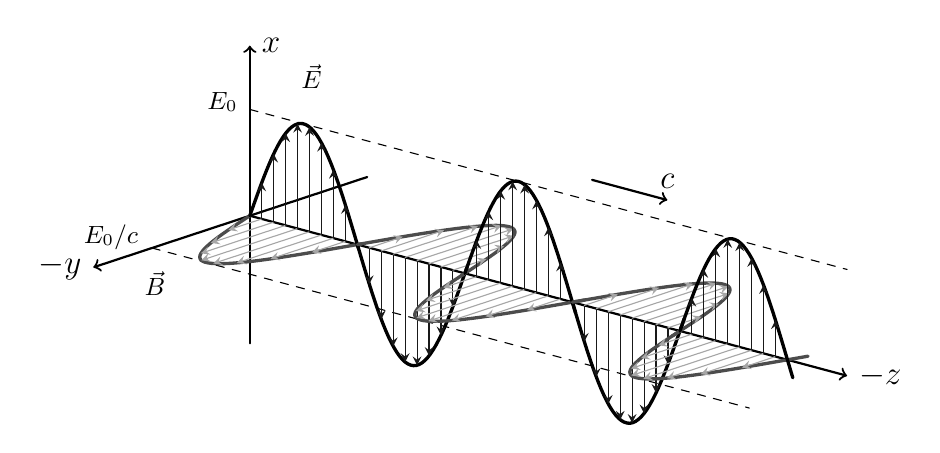
\begin{tikzpicture}[x=(-15:0.9), y=(90:0.9), z=(-150:1.1),
        line cap=round, line join=round,
        axis/.style={black, thick,->},
        axis2/.style={black},
        axis3/.style={black, thick, <-},
        vector/.style={>=stealth,->}]
        \large
        \def\A{1.5}
        \def\nNodes{5} % use even number
        \def\nVectorsPerNode{8}
        \def\N{\nNodes*40}
        \def\xmax{\nNodes*pi/2*1.01}
        \pgfmathsetmacro\nVectors{(\nVectorsPerNode+1)*\nNodes}
        \def\vE{{\color{Ecol}\mathbf{E}}}
        \def\vB{{\color{Bcol}\mathbf{B}}}

        \def\drawENode{ % draw E node and vectors with some offset
        \draw[Ecol,very thick,variable=\t,domain=\iOffset*pi/2:(\iOffset+1)*pi/2*1.01,samples=40]
        plot (\t,{\A*sin(\t*360/pi)},0);
        \foreach \k [evaluate={\t=\k*pi/2/(\nVectorsPerNode+1);
                \angle=\k*90/(\nVectorsPerNode+1);}]
        in {1,...,\nVectorsPerNode}{
        \draw[vector,EVcol]  (\iOffset*pi/2+\t,0,0) -- ++(0,{\A*sin(2*\angle+\iOffset*180)},0);
        }
        }
        \def\drawBNode{ % draw B node and vectors with some offset
        \draw[Bcol,very thick,variable=\t,domain=\iOffset*pi/2:(\iOffset+1)*pi/2*1.01,samples=40]
        plot (\t,0,{\A*sin(\t*360/pi)});
        \foreach \k [evaluate={\t=\k*pi/2/(\nVectorsPerNode+1);
                \angle=\k*90/(\nVectorsPerNode+1);}]
        in {1,...,\nVectorsPerNode}{
        \draw[vector,Bcol!50]  (\iOffset*pi/2+\t,0,0) -- ++(0,0,{\A*sin(2*\angle+\iOffset*180)});
        }
        }

        % MAIN AXES
        \draw[axis] (0,0,0) -- ++(\xmax*1.1,0,0) node[right] {$-z$};
        \draw[axis2, dashed] (0,1.5,0) -- ++(\xmax*1.1,0,0) node[right] {$ $};
        \draw[axis2, dashed] (0,0,1.5) -- ++(\xmax*1.1,0,0) node[right] {$ $};
        \draw[axis] (0,-\A*1.2,0) -- (0,\A*1.6,0) node[right] {$x$};
        \draw[axis] (0,0,-\A*1.2) -- (0,0,\A*1.6) node[left] {$-y$};


        % draw (anti-)nodes
        \foreach \iNode [evaluate={\iOffset=\iNode-1;}] in {1,...,\nNodes}{
        \ifodd\iNode \drawBNode \drawENode % E overlaps B
        \else        \drawENode \drawBNode % B overlaps E
        \fi
        }
        \node[black] at (0.9,2.2,0) {\small $\vec{E}$};
        \node[black] at (0.9,0,2.4) {\small $\vec{B}$};
        \node[black] at (-0.4,1.5,0) {\small $E_0$};
        \node[black] at (-0.6,0,1.5) {\small $E_0/c$};
        \draw[axis] (5,1.8,0) -- ++(1.1,0,0) node[above] {$c$};

    \end{tikzpicture}
\end{center}

$\vE$ dan $\vB$ sefasa dan saling tegak lurus; amplitudo (real) keduanya berhuungan dalam persamaan:
\begin{align*}
    B_0=\frac{k}{\omega}E_0=\frac{1}{c}E_0
\end{align*}

Maka, intensitas medan magnet berdasarkan persamaan yang telah diketahui ($\vE =100 \cos{(\omega t +8 z)\hat{i}}$) adalah
\begin{align*}
    \vB(z,t)&=B_0 \cos{(\omega t +8 z)}\ -\hat{j}\\
    &=\frac{1}{c}E_0 \cos{(\omega t +8 z)}\ -\hat{j}\\
    &=\frac{1}{3\times 10^8}100 \cos{(\omega t +8 z)}\ -\hat{j}\\
    \vB(z,t)&=3.33 \times 10^{-7} \cos{(\omega t +8 z)}\ -\hat{j}
\end{align*} 
        \end{answer}
    \end{enumerate}

\end{enumerate}
\end{document}

